\chapter{Regularity}

\section{The $T_3$ axiom}

\begin{framed}
  \begin{df}[$T_3$]
    A~topological space~$X$ is \emph{regular\/} (or satisfies the~$T_3$
    \emph{axiom\/}) when
    \begin{center} \it
      for any $x\in X$ and any closed $A \not\owns x$ there are disjoint open
      $V_1, V_2$ such that $V_1\owns x$ and $V_2\supseteq A$.
    \end{center}
  \end{df}
\end{framed}

\begin{figure}[h]
  \centering
  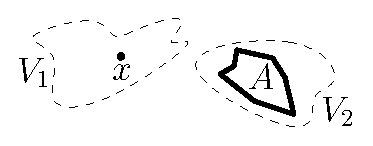
\includegraphics[height=13mm]{../img/t3.eps}
  \caption{$T_3$ property}
\end{figure}

Even though the definition concerns points, it may be reformulated without
them.

\begin{prop} \label{topreg-char}
  A space $X$ is regular iff each $U\in \Omega(X)$ can be described as
  \[
    U = \bigcup \{V\in \Omega(X) \st \overline{V} \subseteq U\}.
  \]
\end{prop}
\begin{proof}
  The inclusion~$\supseteq$ is obvious.

  $\Rightarrow$:
  Choose an~$x\in U$.
  Since $A := X\setminus U \not\owns x$ is closed, the existence
  of~$V_1$~and~$V_2$ from $(T_3)$ is stipulated.
  The disjointedness $V_1 \cap V_2 = \none$ leads to $V_1\subseteq X\setminus
  V_2$, which is a closed set.
  Therefore, $\overline{V_1}\subseteq X\setminus V_2$.

  Furthermore, the relation $A\subseteq V_2$ is equivalent to the relation
  $X\setminus V_2\subseteq X \setminus A = U$.
  Hence, for $V_x := V_1$ one has $\overline{V_x}\subseteq X\setminus V_2\subseteq
  U$.
  Such a~system $\{V_x \st x\in U\}$ constitutes a~subset cover of $U$, and
  consequently, finishes the proof of~the~inclusion $\subseteq$.

  $\Leftarrow$:
  With $U := X\setminus A$ take $V_x$ from above and set $V_1 := V_x$ and $V_2
  := X\setminus \overline{V_x}$.
\end{proof}

Now we will deal with the~closure in the~formula:

\begin{lem} \label{lem:rb-char}
  $\overline{V}\subseteq U \quad \equiv \quad \exists W\in \Omega(X)\colon W \cap V =
  \none \;\; \& \;\; W \cup U = X$.
\end{lem}
\begin{proof}
  $\Rightarrow$:
  Take $W := X\setminus \overline{V}$.

  $\Leftarrow$:
  Recall closure's definition.
  Suppose $z\in \overline{V}\setminus U$.
  Since $W \cup U = X$, the $z$ must lie in the $W$.
  Howbeit, the $W$ does not intersect the $V$---making $z\not\in \overline{V}$.
\end{proof}

Without loss of generality, the $W$ may be replaced by~the
pseudocomplement~$V^*$ in~$\Omega(X)$, that is, by the open set $X\setminus
\overline{V}$.

\begin{rem}
Pseudocomplements always exist in frames:
setting
\[
  a^* := \bigvee \{x \st x \wedge a = 0\},
\]
we have
\[
  a^* \wedge a = \bigvee \{x \st x \wedge a = 0\} \wedge a = \bigvee \{x \wedge
  a \st x \wedge a = 0\} = 0
\]
(the second equality from the frame distributivity), and hence thus defined
$a^*$ is~the~largest $x$ such that $a \wedge x = 0$.
\end{rem}

\section{Regular locales}

\begin{framed}
  \begin{nota}[$\rb$]
    \[
      V \rb U \quad \equiv \quad V^* \vee U = 1,
    \]
    which is referred to by stating that \emph{``V is rather below U''\/}.
  \end{nota}
\end{framed}

\begin{lem} \label{rb->leq}
  $a \rb b \Rightarrow a \leq b$.
\end{lem}
\begin{proof}
  Using~distributivity, we have
  \[
    a = a \wedge 1 = a \wedge (a^* \vee b) = (a \wedge a^*) \vee (a \wedge b) =
    0 \vee (a \wedge b) = a \wedge b. \qedhere
  \]
\end{proof}

With $\rb$ notation we are able to adopt the characterization~\ref{topreg-char}
by~defining regularity as~follows:
\begin{framed}
  \begin{df}[Reg]
    A locale is called \emph{regular\/} if
    \[
      a = \bigvee \{x \st x \rb a\}
    \]
    for all its elements $a$.
  \end{df}
\end{framed}

Thus, we observe that
\begin{center} 
  \emph{a topological space $X$ is regular iff $\Omega(X)$ is regular.\/}
\end{center}

\section{Strength of regularity}

\begin{lem} \label{oplus-vee-distrib}
  ~
  \begin{enumerate}
  \item $\bigvee_{i\in J} \left(a_i \oplus b\right) = \left(\bigvee_{i\in J}
    a_i \right) \oplus b$.
  \item $\bigvee_{i\in J} \left(a \oplus b_i\right) = a \oplus
    \left(\bigvee_{i\in J} b_i \right)$.
  \item $\left(\bigvee_{i\in J} a_i\right) \oplus \left(\bigvee_{j\in J}
    b_j\right) = \bigvee_{i, j\in J} \left(a_i \oplus b_j\right)$.
  \end{enumerate}
\end{lem}
\begin{proof}
  (i):
  Recall \ref{oplus-iota} on page~\pageref{oplus-iota}\thinspace.
  We have
  \begin{align*}
    \left(\bigvee_{i\in J} a_i \right) \oplus b
    &= \iota_1\left(\bigvee_{i\in J} a_i \right) \wedge \iota_2(b)
    = \left(\bigvee_{i\in J} \iota_1(a_i) \right) \wedge \iota_2(b) \\
    &= \bigvee_{i\in J} \left(\iota_1(a_i) \wedge \iota_2(b) \right)
    = \bigvee_{i\in J} \left(a_i \oplus b\right)
  \end{align*}
  as frame homomorphisms $\iota_i$ preserve suprema (for the second equality)
  and as the binary meet commutes with joins in frames (for the third
  equality).

  (ii):
  Analogously by symmetry.

  (iii):
  By consecutive application of (i) and (ii).
\end{proof}

\begin{lem}
  For a general locale $L$ and any of its saturated $U\in \left\uparrow
  d_L\right.$
  \[
    (a \wedge b, a \wedge b) \in U \qquad \Longrightarrow \qquad \forall x \rb
    a, \, y \rb b: \; (x, y) \in U
  \]
\end{lem}
\begin{proof}
  Beginning with $(x, y)\in x \oplus y$, we rewrite
  \begin{align*}
    x \oplus y &= (x \wedge (y^* \vee b)) \oplus (y \wedge (x^* \vee a)) \\
               &= (\; (x \wedge y^*) \; \vee \; (x \wedge b) \; ) \oplus (\; (y
    \wedge x^*) \; \vee \; (y \wedge a) \; )
  \end{align*}
  (using ``rather-belowness'' and distributivity, respectively).

  Proceeding with (iii) of Lemma~\ref{oplus-vee-distrib}\thinspace,
  \begin{align*}
     \ldots = \; &(\; (x \wedge y^*) \oplus (y \wedge x^*) \; ) \vee 
            (\; (x \wedge y^*) \oplus (y \wedge a) \; ) \; \vee \\
            \vee \; &(\; (x \wedge b) \oplus (y \wedge x^*) \; ) \vee
            (\; (x \wedge b) \oplus (a \wedge y) \; ) \\
     \subseteq \; &(y^*\oplus y) \vee (y^*\oplus y) \vee (x\oplus x^*) \vee (\;
            (a \wedge b)\oplus(a \wedge b) \;)
  \end{align*}
  where the upper-bound of the last member follows
  from~\ref{rb->leq}\thinspace.

  Besides, the ultimate expression is a subset of $U$:
  as $(x^*\oplus x), (y^*\oplus y)\subseteq d_L$ and $(a \wedge b)\oplus(a
  \wedge b)\subseteq U$ from the premise.
  In conclusion, $(x, y)\in x \oplus y \subseteq U$.
\end{proof}

\begin{thm}
  (Reg) implies (I-Haus).
\end{thm}
\begin{proof}
  We will show that regular locales satisfy \eqref{eq:meets-in-satur}\thinspace
  from~\ref{meets-in-satur} (see page~\pageref{meets-in-satur}).
  Let $(a \wedge b, a \wedge b) \in U$.
  By the previous lemma, we have $(x, y)\in U$ with $x \rb a$ and $y \rb b$.
  Recall the saturatedness on~page~\pageref{df:satur}\thinspace.
  Since $U$ is saturated,
  \[
    \left\{ (x, y) \st x \rb a \right\} \subseteq U
    \Longrightarrow
    \left(\bigvee \{x \st x \rb a\}, y\right)\in U,
  \]
  or equally, using regularity,
  \[
    \left(a, y\right)\in U
  \]
  for all $y \rb b$.
  Therefore, in the same way:
  $(a, b) = \left(a, \bigvee \{y \st y \rb b\}\right)\in U$.
\end{proof}

By Theorem~\ref{IHaus->DSHaus} on page~\pageref{IHaus->DSHaus}\thinspace, we
obtain
\begin{cor}
  (Reg) implies (DS-Haus).
\end{cor}

It is useful to characterize (Reg) by a formula that resembles (Sfit):
\begin{lem} \label{reg-char}
  A locale is regular iff
  \[
    a \not\le b \qquad \Rightarrow \qquad \exists c: \quad a \vee c = 1 \quad
    \& \quad c^* \not\leq b.
  \]
\end{lem}
\begin{proof}
  $\Rightarrow$:
  Suppose $a \not\le b$;
  using regularity, there is $x \rb a$ with $x \not\le b$ (otherwise $\bigvee
  \{x \st x \rb a\} \le b$).
  Let $c := x^*$.
  In other words, $x \rb a$ leads to $a \vee c = a \vee x^* = 1$.
  Additionally, $c^* \not\le b$:
  or~otherwise (from a~standard pseudocomplement property) $x \le x^{**} = c^*
  \le b$.

  $\Leftarrow$:
  By~\ref{rb->leq} we always have the inequality $\bigvee \{x \st x \rb a\} \le
  a$.
  Hence, for contradiction let us assume $a \not\le \bigvee \{x \st x \rb a\}$.
  Then there exists $c$ from the~premise.
  Specifically, $1 = a \vee c \le a \vee c^{**}$, which gives us $c^* \rb a$;
  and yet $c^* \not\le \bigvee \{x \st x \rb a\}$.
\end{proof}

\begin{thm} \label{thm:reg->sfit}
  (Reg) implies (Sfit).
\end{thm}
\begin{proof}
  Let $a \not\le b$.
  From Lemma~\ref{reg-char}\thinspace, we get an~element $c$ such that $a \vee
  c = 1$ and $c^* \not\le b$.
  What is more, it satisfies $b \vee c \ne 1$.
  If not so then by~distributivity
  \[
    b = b \vee 0 = b \vee (c \wedge c^*) = (b \vee c) \wedge (b \vee c^*) = 1
    \wedge (b \vee c^*) = b \vee c^*,
  \]
  which contradicts $c^* \le b$.
\end{proof}

\begin{rem}
  By Theorem~\ref{thm:what-does-sfit-do} on
  page~\pageref{thm:what-does-sfit-do}, (Reg) implies all Hausdorff type axioms
  mentioned in Chapter IV.
\end{rem}

\begin{prop} \label{prop:sloc-of-reg}
  Every sublocale $S$ of a~regular locale $L$ is also regular.
\end{prop}
\begin{proof}
  Let $h\colon L \to S$ be a~frame homomorphism.
  By~\ref{lem:rb-char}, we can formulate ``rather-belowness'' as
  \[
    a \rb b 
    \; \equiv \;
    \exists c, \; a \wedge c = 0 \text{ and } c \vee b = 1,
  \]
  Since $h(a) \wedge h(c) = h(a \wedge c) = 0$ and $h(c) \vee h(b) = h(c \vee
  b) = 1$, we have $a \rb b \Rightarrow h(a) \rb h(b)$.
  Thus, $\{ h(x) \st x \rb a\} \subseteq \{ y \st y \rb h(a)\}$, and hence,
  $
    h(a)
    = h (\bigvee \{ x \st x \rb a\})
    = \bigvee \{ h(x) \st x \rb a\}
    \le \bigvee \{ y \st y \rb h(a) \}.
  $
  The other inequality is from~\ref{rb->leq}.

  Because a~sublocale homomorphism $h$ is onto, for any $b\in S$ there is $a\in
  L$ such that
  $
    b
    = h(a)
    = \bigvee \{ y \st y \rb h(a) \}
    = \bigvee \{ y \st y \rb b \}.
  $
\end{proof}

\begin{rem}[Fitness]
  Unlike the regularity, the subfitness is not hereditary:
  in~general, not every sublocale of a~subfit locale is subfit.
  The hereditary subfitness is called \emph{fitness\/}, and by
  Proposition~\ref{prop:sloc-of-reg} and Theorem~\ref{thm:reg->sfit}, we have
\end{rem}
\begin{obs}
  (Reg) implies the fitness.
\end{obs}
